% \glsresetall
\chapter{Webpack Module Federation} % Main chapter title
\label{Chapter5}

\lhead{Chapter 5. \emph{Webpack Module Federation}}

A rather new way of creating micro frontends is the \textbf{Webpack 5 Module Federation (WMF)}. With the release of version 5 on October 10, 2020, this technology added certain features which improved its usage for developing micro frontends.\cite{wmf_concepts}
The way it does that, is via modularizing self-compiled code parts and publishing them for integration by other modules. This published modules can be micro frontends themselves and are called \textbf{remotes} whereas the integrating modules are called \textbf{hosts}. 
\textbf{Hosts} refer to \textbf{remotes} under a configured name. This name is not actually known to the \textbf{host} during the compile time, but is first resolved at runtime.
The self-compiled \textbf{remote} in this case can be anything, a micro frontend or some sort of utility script. This way the Module Federation provides a way to avoid external or manual script loading and instead gives opportunities to automatically lazy load necessary code blocks during runtime.\cite{wmf_concepts}
The usage of the WMF is tied to the Webpack bundler, since the necessary configuration is done in the \texttt{webpack.config.js}. This restriction is applied to every \textbf{remote} in the WMF landscape, not only to the \texttt{host}.

Since the main focus of this document is to propose methods of avoiding redundancies in micro frontend landscapes, an introduction of this WMF feature is given here.
WMF can be used in combination with most of the common UI Frameworks. Since the implementation for this thesis was done with Angular, the further examples and explanations will be Angular-based.

\section{Enabling the Module Federation}

Prior to introducing the usage of the Module Federation, it is necessary to introduce Webpack itself first, as it is a mandatory feature for using the Module Federation. Popular UI frameworks like React, VueJS or Angular use Webpack under the hood anyway, so it isn't as much of a restriction as it seems.\cite{webpack_angular}\cite{webpack_react}\cite{webpack_vue}
The documentation of the named frameworks imply that Webpack is used by default, but can be customized if necessary by the developer.

For Angular in particular, it is necessary to install two dependencies via the Angular CLI, to enable the features of the Module Federation. The command used for this is shown in \ref{list:angluar_wmf_command}. 

\begin{lstlisting}[language=Bash, caption=Angular CLI console command to enable Module Federation in an Angular project, label=list:angluar_wmf_command,  xleftmargin=.0\textwidth, xrightmargin=.0\textwidth]
	ng add @angular-architects/module-federation --project name --port port
\end{lstlisting}

These commands enable the Module Federation for an Angular project. Since the CLI protects the Webpack configuration from access, a custom builder is required. The \texttt{@angular-architects/module-federation} package provides exactly that.
After installing this dependency in an Angular project, a \texttt{webpack.config.js} will appear on root level of the corresponding project.\cite{wmf_angular_dependency_install}
This dependency has to be added in each \textbf{remote} or \textbf{host} of the WMF landscape. 

After enabling the Module Federation inside a project, the necessary configuration can be applied to the \texttt{webpack.config.js} file. The \textbf{remotes} publish their modules and \textbf{hosts} consume them. Thus a developer can distinguish what module has which role.

\section{Shared dependency feature}

As noted before WMF is a micro frontend framework, which offers means to solve the issue of redundant libraries in its landscapes.
This feature is enabled and configured, as well as the rest of the WMF, via the \texttt{webpack.config.js}. When configuring the components of the landscape, it is possible to define a section where shared dependencies are described. These dependencies can be defined in different ways. For instance, it is possible to define a strict version of the dependency, which would result in the framework loading this specific version. Or one can define a less restricted dependency, which would mean that if another \texttt{remote} loads the same dependency but in a different version, the framework would automatically apply the highest major version of the dependency to both micro frontends.

\begin{lstlisting}[language=JavaScript, caption=Example of sharing dependencies configured in the \texttt{webpack.config.js}, label=list:shared_mapping_wmf,  xleftmargin=.01\textwidth, xrightmargin=.01\textwidth]
	shared: share({
		"@angular/core": { 
			singleton: true, 
			strictVersion: false, 
			requiredVersion: '12.2.0' 
		},
		"@angular/common": { 
			singleton: true, 
			strictVersion: false, 
			requiredVersion: '12.2.0' 
		},
		"@fundamental-ngx/core": { 
			singleton: true, 
			strictVersion: false, 
			requiredVersion: '0.33.0-rc.214' 
		},
		
		...sharedMappings.getDescriptors()
	})
\end{lstlisting}

Listing \ref{list:shared_mapping_wmf} is an example of how to share libraries in a restrictive way. To provide a less restricted configuration, a simple array of the shared dependency names suffices. But to ensure a redundant free landscape, these restrictions are necessary. Each configuration property will be explained below.

\begin{itemize}
	\item \texttt{singleton} - This property defines if the dependency should be able to be loaded more than once in different versions or not. If set to \texttt{true}, WMF will automatically pick the highest version of a major release of this dependency available and distribute it to the \textbf{remotes}.\cite{wmf_version_mismatch}
	
	\item \texttt{strictVersion} - This property defines if the dependency requires a specific version to work. If set to \texttt{true} WMF, will load the required version even if another dependency mapping with the same name is present. This can lead to conflicts with the \texttt{singleton} property, if configured poorly.
	
	\item \texttt{requiredVersion} - This property defines the required version of the dependency. When working with a package manager (e.g. NPM), this version has to be aligned with the locally installed version of the dependency. If the \texttt{strictVersion} property is set to \texttt{false}, this property defines the minimum version for the micro frontend. 
	
	It has to be mentioned that WMF is able to distinguish between major releases. If a higher version of the same major release is available, it will be loaded (e.g. \texttt{@angular/common@12.3.1}). For instance, if the next higher version is of a different major release e.g. 13.X.X, WMF would not consider to load it for the \textbf{remotes} which have the \texttt{requiredVersion} of release 12.X.X configured.
\end{itemize}

Now, when it comes to sharing the dependencies inside the micro frontend landscape, each \textbf{remote} has to participate. That means each micro frontend has to define its required dependencies in their respective versions. Additionally, it has to be mentioned that the micro frontends themselves have to use dynamic imports when importing shared dependencies. Through the asynchronous behavior of the import, Webpack has time to pick the correct version of the dependency inside the landscape.\cite{wmf_concepts}
Analyzing this statement in combination with the information taken from \ref{list:shared_mapping_wmf}, it becomes obvious that multiple versions of the same framework can exist in a landscape. 

\section{Multi-version landscapes in WMF}

Figure \ref{fig:wmf_multiversions} illustrates the case, of how WMF handles a multi-version landscape.

\begin{figure}[!h]
	\centering
	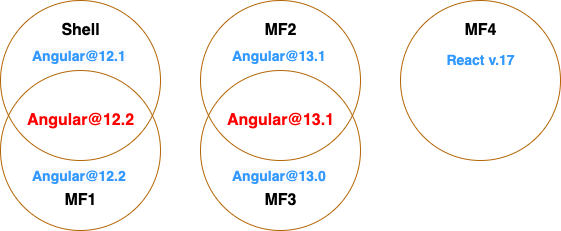
\includegraphics[width=0.7\textwidth]{Figures/multi_version_diagramm.drawio.png}
	\caption{WMF way of handling multi-versions}
	\label{fig:wmf_multiversions}
\end{figure}

As it can be seen, WMF always picks the latest major release, assuming the respective micro frontends have a similar configuration as shown in listing \ref{list:shared_mapping_wmf} applied. If, for instance, \textbf{MF3} has its \texttt{strictVersion} property set to \texttt{true}, it would cause the loading of its libraries too.

There are side effects to sharing the same dependency over the whole micro frontend landscape. One of which is the increase in bundle sizes, since every \textbf{remote} bundles its local dependencies. WMF then picks the one to serve during the runtime of the landscape.
This impact has a trade-off tough. Returning users can benefit from cached dependencies.\cite{wmf_multi_versions}

Integrating several \textbf{remotes} using the same dependencies leads to the issue of redundancies, which WMF is able to resolve. Via configuration of shared dependencies WMF provides a way to reduce redundant libraries in its landscape.